\documentclass{beamer}


\usepackage[english]{babel}
\usepackage[utf8]{inputenc}
\usepackage{amsmath,amssymb,amsfonts,amsthm}
\usepackage{stmaryrd}
\usepackage{hyperref}  % automagically makes clickable references, table of contents
\usepackage{enumerate}
\usepackage{lipsum}
\usepackage{graphicx}
\usepackage{wrapfig}
\usepackage{pifont}
\usepackage{epigraph}

\usepackage{tikz}
\usetikzlibrary{matrix, fit, positioning, decorations.pathmorphing, decorations.pathreplacing}
\tikzset{
	edge/.style={thick, ->},
	table nodes/.style={
		rectangle,
		draw=black,
		style=thick,
		align=center,
		minimum height=7mm,
		text depth=0.5ex,
		text height=2ex,
		inner xsep=0pt,
		outer sep=0pt,
		inner sep=0pt
	},
	table/.style={
		matrix of nodes,
		row sep=-0.5pt,
		column sep=-0.5pt,
		nodes={
			table nodes
		}
	}
}


% Sets and set operations
\newcommand{\R}{\mathbb{R}} % the reals
\newcommand{\Z}{\mathbb{Z}} % the integers
\newcommand{\N}{\mathbb{N}} % the natural numbers
\renewcommand{\O}[1]{\mathcal{O}\l(#1\r)}
%\newcommand{\pot}[1]{\mathcal{P}(#1)} % power set

% Other operators
%\renewcommand{\mod}{\operatorname{\%}}
\newcommand{\s}{\ast}

% Convenience
\renewcommand{\l}{\left} % short left
\renewcommand{\r}{\right} % short right
\newcommand{\pfrac}[2]{\l( \frac{#1}{#2} \r)}
\newcommand{\divmod}{\overset{\operatorname{divmod}}{\longrightarrow}}
\newcommand{\code}[1]{\texttt{#1}}


\newcommand{\trienode}[2]{% node label, options for matrix
	\matrix (n#1) [table, text width=7mm, ampersand replacement=\&, #2]
	{ #1 \& {} \& {} \& {} \& {} \\};
	\node[font=\tiny, anchor=south] at (n#1-1-2.north) {0};
	\node[font=\tiny, anchor=south] at (n#1-1-3.north) {1};
	\node[font=\tiny, anchor=south] at (n#1-1-4.north) {2};
	\node[font=\tiny, anchor=south] at (n#1-1-5.north) {3}
}


\newcommand{\itemspacing}[1]{\setlength\itemsep{#1}}

%\setbeamertemplate{bibliography item}{\insertbiblabel}
\setbeamertemplate{footline}[frame number]




\title{Storing a Sparse Table}
\subtitle{Seminar Theory of Efficient Hashing Techniques}
\date{21.07.2016}
\author{Simon Feiden}


\begin{document}
	
	
\maketitle

\begin{frame}
	\tableofcontents
\end{frame}


\section{Introduction}
In this work, we elaborate and explain the techniques presented in \cite{tarjan:storing_sparse_table} to store a map from words to objects with $\O{1}$ lookup and minimised storage needs.
The words are natural numbers in the range $0$ through $N-1$ while the objects can be arbitrary data.
We consider the \emph{static case} where $n$ words are added to the map before any lookups are performed.
In order to apply several optimisations to our storage scheme, we assume that $N$ is bounded by a polynomial in $n$, i.e.~$N \in \O{n^c}$.
This guarantees that the tables we will compress are sparse, but not too sparse.
Use cases are LR parsing and sparse Gaussian elimination which can be implemented using such tables.
In both cases, $c = 2$ giving $N \in \O{n^2}$. \\
First of all, we will introduce \emph{tries} which are a data structure based on trees.
Then, seemingly unrelated, we will present a way to compress tables in three steps using row and column displacements as well as a special indexing scheme.
Finally, we combine both ideas to obtain a way to store a sparse table with good space complexity.


\section{Tries}
\begin{frame}{Tries --- Overview}
	\begin{itemize}[<+->]
		\itemspacing{20pt}
		\item Tree data structure for integers
		\item Also known as \emph{prefix trees} for strings
		\item Degree $k$ at every node
		\item Usual operations: \code{insert}, \code{lookup}, \code{delete}
		\item Path in trie specified by a single integer
	\end{itemize}
\end{frame}


\newcommand{\trienode}[2]{% node label, options for matrix
	\matrix (n#1) [table, text width=7mm, ampersand replacement=\&, #2]
	{ #1 \& {} \& {} \& {} \& {} \\};
	\node[font=\tiny, anchor=south] at (n#1-1-2.north) {0};
	\node[font=\tiny, anchor=south] at (n#1-1-3.north) {1};
	\node[font=\tiny, anchor=south] at (n#1-1-4.north) {2};
	\node[font=\tiny, anchor=south] at (n#1-1-5.north) {3}
}

\begin{frame}{Examples --- \code{insert}}
	\resizebox{\textwidth}{!}{%
		
		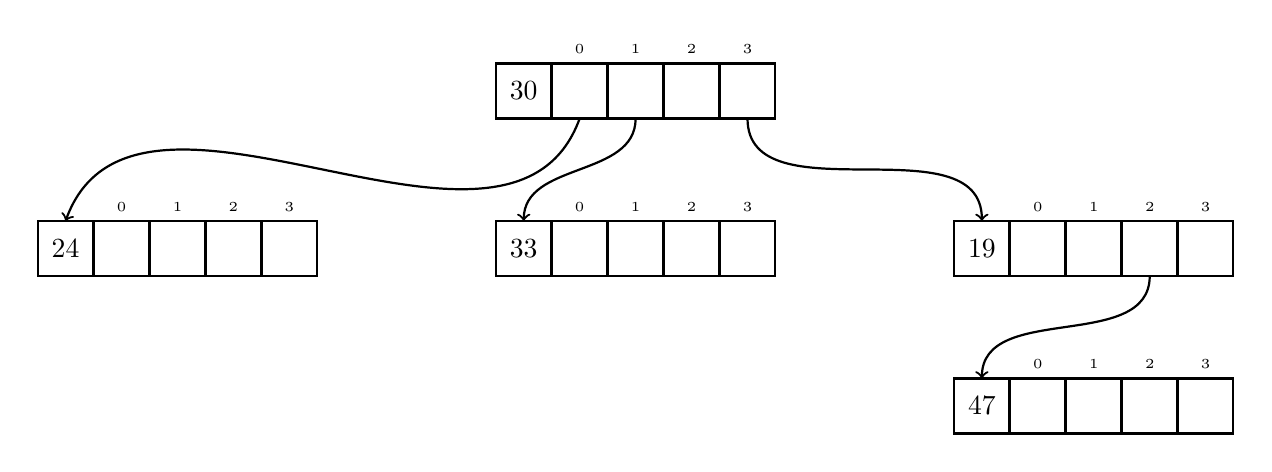
\begin{tikzpicture}[align=center, node distance=2cm]
			\trienode{30}{};
			
			\trienode{33}{below of=n30};
			\draw[edge] (n30-1-3.south) to[out=270, in=90] (n33-1-1.north);
			
			\visible<3->{
				\trienode{24}{left =2cm of n33};
				\draw[edge] (n30-1-2.south) to[out=250, in=70] (n24-1-1.north);
			}
			
			\visible<5->{
				\alert<6-7>{ \trienode{19}{right=2cm of n33}; }
				\draw[edge] (n30-1-5.south) to[out=270, in=90] (n19-1-1.north);
			}
			
			\visible<8->{
				\trienode{47}{below of=n19};
				\draw[edge] (n19-1-4.south) to[out=270, in=90] (n47-1-1.north);
			}
		\end{tikzpicture}
	}
	
	\begin{itemize}
		\item<2-> $24 \divmod (6, 0)$
		\item<4-> $19 \divmod (4, 3)$
		\item<6-> $47 \divmod (11, 3) \uncover<7->{ \divmod (2, 3) }$
	\end{itemize}
	
\end{frame}


\begin{frame}{Examples --- \code{lookup}}
	\resizebox{\textwidth}{!}{%
		
		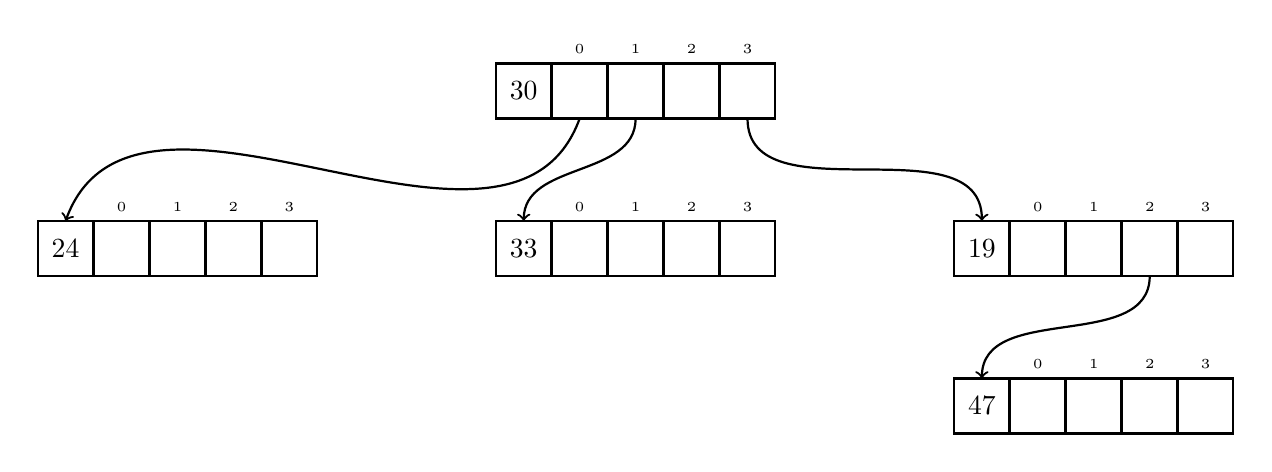
\begin{tikzpicture}[align=center, node distance=2cm]
		\alert<2,7>{
			\trienode{30}{};
		}
		
		\alert<9>{
			\trienode{33}{below of=n30};
			\draw[edge] (n30-1-3.south) to[out=270, in=90] (n33-1-1.north);
		}
		
		\alert<4>{
			\trienode{24}{left =2cm of n33};
			\draw[edge] (n30-1-2.south) to[out=250, in=70] (n24-1-1.north);
		}
		
		\trienode{19}{right=2cm of n33};
		\draw[edge] (n30-1-5.south) to[out=270, in=90] (n19-1-1.north);
		
		\trienode{47}{below of=n19};
		\draw[edge] (n19-1-4.south) to[out=270, in=90] (n47-1-1.north);
		\end{tikzpicture}
	}
	
	\begin{itemize}
		\item<2-> $24
				\uncover<3->{ \divmod (6, 0) }
				\phantom{mmm}$
				\uncover<5->{ \ding{51} }
				
		\item<6-> $25
				\uncover<8->{ \divmod (6, 1) }
				\uncover<10->{ \divmod (1, 2) }
				\phantom{mmm}$
				\uncover<11>{ \ding{55}}
	\end{itemize}
	
\end{frame}


\begin{frame}{Examples --- \code{delete}}
	\resizebox{\textwidth}{!}{%
		
		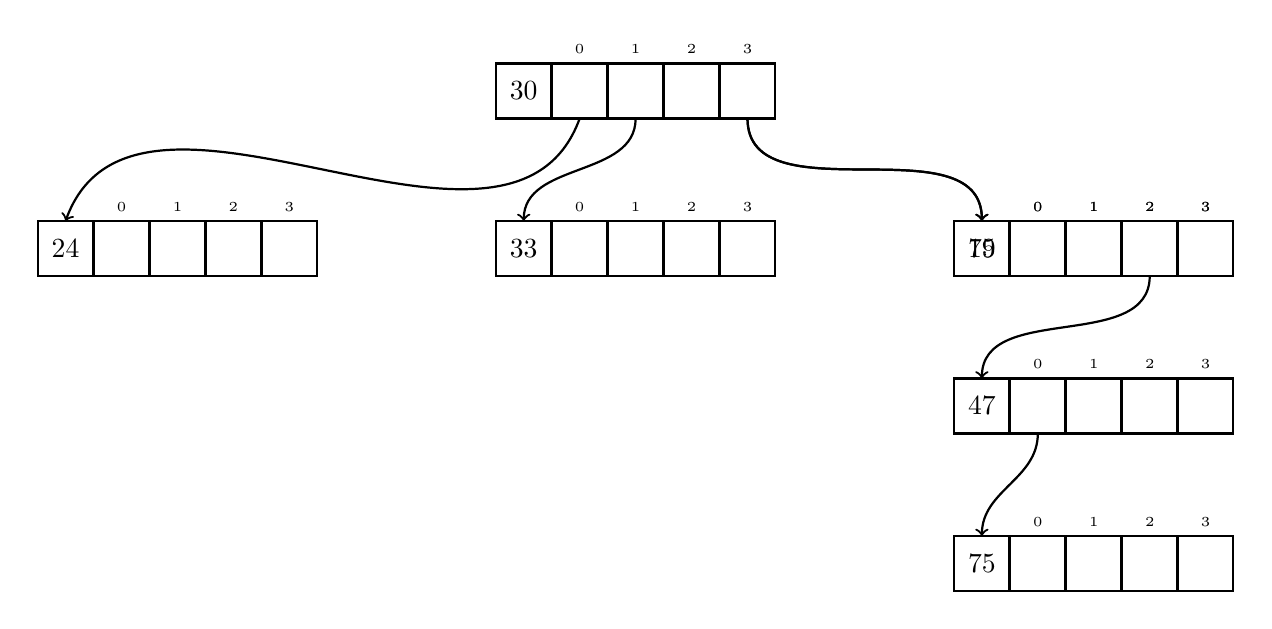
\begin{tikzpicture}[align=center, node distance=2cm]
		\trienode{30}{};
		
		\trienode{33}{below of=n30};
		\draw[edge] (n30-1-3.south) to[out=270, in=90] (n33-1-1.north);
		
		\visible<1-2>{
			\alert<2>{
				\trienode{24}{left =2cm of n33};
				\draw[edge] (n30-1-2.south) to[out=250, in=70] (n24-1-1.north);
			}
		}
		
		\visible<-6>{
			\alert<4,6-7>{
				\trienode{19}{right=2cm of n33};
				\draw[edge] (n30-1-5.south) to[out=270, in=90] (n19-1-1.north);
			}
		}
		
		\visible<7->{
			\alert<7->{
					\matrix (n75b) [table, text width=7mm, ampersand replacement=\&, right=2cm of n33]
						{ 75 \& {} \& {} \& {} \& {} \\};
					\node[font=\tiny, anchor=south] at (n75b-1-2.north) {0};
					\node[font=\tiny, anchor=south] at (n75b-1-3.north) {1};
					\node[font=\tiny, anchor=south] at (n75b-1-4.north) {2};
					\node[font=\tiny, anchor=south] at (n75b-1-5.north) {3};
					\draw[edge] (n30-1-5.south) to[out=270, in=90] (n75b-1-1.north);
			}
		}
		
		\trienode{47}{below of=n19};
		\draw[edge] (n19-1-4.south) to[out=270, in=90] (n47-1-1.north);
		
		\visible<1-5>{
			\alert<5> {
				\trienode{75}{below of=n47};
				\draw[edge] (n47-1-2.south) to[out=270, in=90] (n75-1-1.north);
			}
		}
		\end{tikzpicture}
	}
	
	\begin{itemize}
		\item<1-> \code{delete} 24
		\item<4-> \code{delete} 19
	\end{itemize}
\end{frame}

\begin{frame}{Tries --- Analysis}
	\begin{itemize}[<+->]
		\itemspacing{20pt}
		\item Insertion of $n$ values in range $0, \ldots, N - 1$
		\item Longest path is $\O{\log_k N}$
		\item \code{insert}, \code{lookup}, \code{delete} follow a path (to a leaf)
		\item Constant time changes to nodes in \code{insert}, \code{delete}
		\item Worst case $\O{\log_k N}$ for all three methods
	\end{itemize}
\end{frame}


\section{Tables and Displacements}
\begin{frame}{Sparse Tables}
	\begin{itemize}[<+->]
		\itemspacing{20pt}
		\item Tables are 2d-arrays with cells $\{1, \ldots, m\} \times \{1, \ldots, m\}$ % or $\{ 1, \ldots, m^2 \}$
		\item $N$ must be the table size
		\item Square tables $\implies$ $N = m \cdot m$
		\item Sparseness: $N \in \O{n^c}$
		\item Goal: compressing a table
	\end{itemize}
\end{frame}

\begin{frame}{Sparse Tables --- Displacements}
		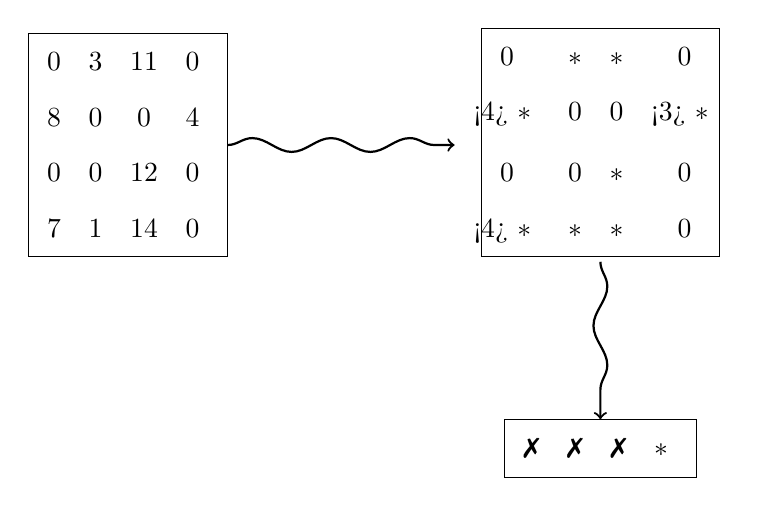
\begin{tikzpicture}[align=center, node distance=6cm]
			\matrix (tbl) [
				matrix of nodes,
				draw=none,
				row sep = 0.7em,
				column sep = 0em,
				ampersand replacement=\&
			] {
				0 \& 3 \& 11 \& 0 \\
				8 \& 0 \&  0 \&  4 \\
				0 \& 0 \& 12 \& 0 \\
				7 \& 1 \& 14 \&  0 \\
			};
			\node[draw, fit = (tbl-1-1) (tbl-4-4)] (tbl-fit) {};
			
			\uncover<2->{
				\matrix (tbl2) [
					matrix of nodes,
					draw=none,
					row sep = 0.7em,
					column sep = 0em,
					ampersand replacement=\&,
					right of = tbl
				] {
					0                 \& $\s$  \& $\s$ \&  0                 \\
					\alert<4>{ $\s$ } \& 0     \& 0    \&  \alert<3>{ $\s$ } \\
					0                 \& 0     \& $\s$ \&  0                 \\
					\alert<4>{ $\s$ } \& $\s$  \& $\s$ \&  0                 \\
				};
				\node[draw, fit = (tbl2-1-1) (tbl2-4-4)] (tbl2-fit) {};
				
				
				\draw[edge, decorate, decoration={snake, segment length = 10mm}] (tbl.east) to (tbl2.west);
			}
			
			\uncover<5->{
				\matrix (clash) [
				matrix of nodes,
				draw=none,
				row sep = 0.7em,
				column sep = 0em,
				ampersand replacement=\&,
				below = 2cm of tbl2
				] {
					\ding{55} \& \ding{55} \& \ding{55} \& $\s$   \\
				};
				\node[draw, fit = (clash-1-1) (clash-1-4)] (clash-fit) {};
				
				
				\draw[edge, decorate, decoration={snake, segment length = 10mm}] (tbl2.south) to (clash.north);
			}
		\end{tikzpicture}
\end{frame}

\begin{frame}{Sparse Tables --- Displacements}
	\centering
	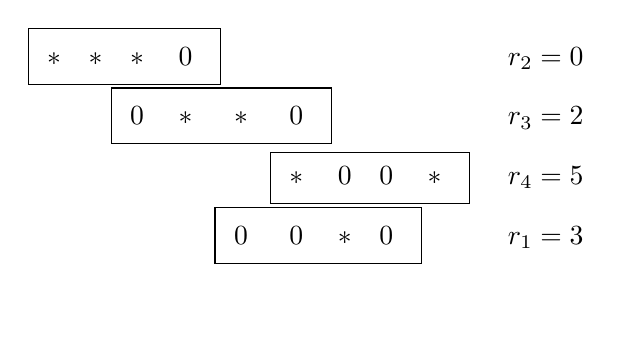
\begin{tikzpicture}[align=center, node distance=2cm]
		\matrix (mx) [%
			matrix of nodes,
			draw = none,
			row sep = 0.7em,
			column sep = 0em,
			ampersand replacement=\&
		] {
			$\s$ \& $\s$ \& $\s$ \& 0    \& {}   \& {}   \& {}   \& {} \& {}   \&[1em] $r_2 = 0$ \\
			{}   \& {}   \& 0    \& $\s$ \& $\s$ \& 0    \& {}   \& {} \& {}   \& $r_3 = 2$ \\
			{}   \& {}   \& {}   \& {}   \& {}   \& $\s$ \& 0    \& 0  \& $\s$ \& $r_4 = 5$ \\
			{}   \& {}   \& {}   \& {}   \& 0    \& 0    \& $\s$ \& 0  \& {}   \& $r_1 = 3$ \\
			$\phantom{5}$ \& $\phantom{6}$ \& $\phantom{7}$ \& $\phantom{10}$ \& $\phantom{11}$ \& $\phantom{13}$ \& $\phantom{3}$ \& $\phantom{0}$ \& $\phantom{16}$ \& $\phantom{r_1 = C}$ \\
		};
		
		\node[draw, fit = (mx-1-1) (mx-1-4)] (1-fit) {};
		\node[draw, fit = (mx-2-3) (mx-2-6)] (2-fit) {};
		\node[draw, fit = (mx-3-6) (mx-3-9)] (3-fit) {};
		\node[draw, fit = (mx-4-5) (mx-4-8)] (4-fit) {};
%		\node[draw, fit = (mx-5-1) (mx-5-9)] (C-fit) {};
	\end{tikzpicture}
	
	\begin{itemize} % placeholder for spacing for next frame
		\item[]
		\item[]
	\end{itemize}
\end{frame}

\begin{frame}{Row Displacements}
	\resizebox{\textwidth}{!}{
		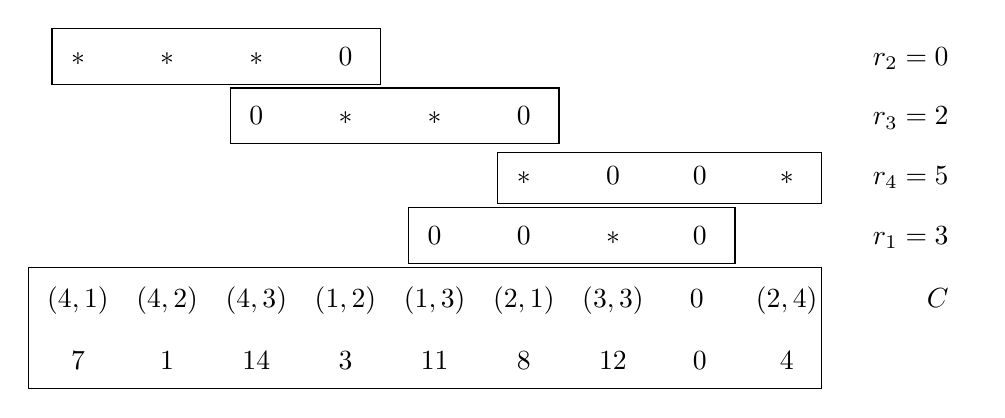
\begin{tikzpicture}[align=center, node distance=2cm]
			\matrix (mx) [%
				matrix of nodes,
				draw = none,
				row sep = 0.7em,
				column sep = 0em,
				ampersand replacement=\&
			] {
				$\s$ \& $\s$ \& $\s$ \& 0    \& {}   \& {}   \& {}   \& {} \& {}   \&[1em] $r_2 = 0$ \\
				{}   \& {}   \& 0    \& $\s$ \& $\s$ \& 0    \& {}   \& {} \& {}   \& $r_3 = 2$ \\
				{}   \& {}   \& {}   \& {}   \& {}   \& $\s$ \& 0    \& 0  \& $\s$ \& $r_4 = 5$ \\
				{}   \& {}   \& {}   \& {}   \& 0    \& 0    \& $\s$ \& 0  \& {}   \& $r_1 = 3$ \\
				$(4,1)$ \&
				$(4,2)$ \&
				$(4,3)$ \&
				$(1,2)$ \&
				$(1,3)$ \&
				$(2,1)$ \&
				$(3,3)$ \&
				$\phantom{(,}0\phantom{0)}$ \&
				$(2,4)$ \&
				$\phantom{r_1 = } C$ \\
				7 \& 1 \& 14 \& 3 \& 11 \& 8 \& 12 \&  0 \&  4 \\
			};
			
			\node[draw, fit = (mx-1-1) (mx-1-4)] (1-fit) {};
			\node[draw, fit = (mx-2-3) (mx-2-6)] (2-fit) {};
			\node[draw, fit = (mx-3-6) (mx-3-9)] (3-fit) {};
			\node[draw, fit = (mx-4-5) (mx-4-8)] (4-fit) {};
			\node[draw, fit = (mx-5-1) (mx-6-9)] (C-fit) {};
		\end{tikzpicture}
	}
	
	\begin{itemize}
		\item<2-> Finding optimal row displacements is NP-complete
		\item<3-> Heuristic approach: sort rows by number of nonnulls
	\end{itemize}
\end{frame}

\begin{frame}{Row Displacements}
	\begin{itemize}[<+->]
		\itemspacing{20pt}
		\item Essential operation on a table: \code{lookup} of key $k$
		\item Calculate position $(i, j)$ for $k$
		\item Check if $C(r_i + j)$ equals $k$
		\item $\O{1}$ lookup in $C$
		\item Single Displacements perform bad in worst case
	\end{itemize}
\end{frame}


\begin{frame}{Indirection}
	\begin{quotation}
		Any problem in computer science can be solved by another layer of indirection.
	\end{quotation}
	\vspace*{-1em}
	\begin{flushright}
		\textup{
		--- David Wheeler
		}
	\end{flushright}
\end{frame}

\begin{frame}{Column Displacements}
	\begin{columns}
		\begin{column}[T]{0.6\textwidth}
			\begin{itemize}[<+->]
				\itemspacing{20pt}
%				\item \makebox[\linewidth][l]{Indirection: Column Displacements}
				\item Indirection: Column Displacements
				\item First displace columns, then displace rows
				\item Fill empty cells with 0
				\item Better compression makes up for more rows
				\item Why it works: fewer nonulls per row
			\end{itemize}
		\end{column}
		
		\begin{column}[T]{0.4\textwidth}
			\centering
			\only<2> {
				\resizebox{0.9\textwidth}{!}{
					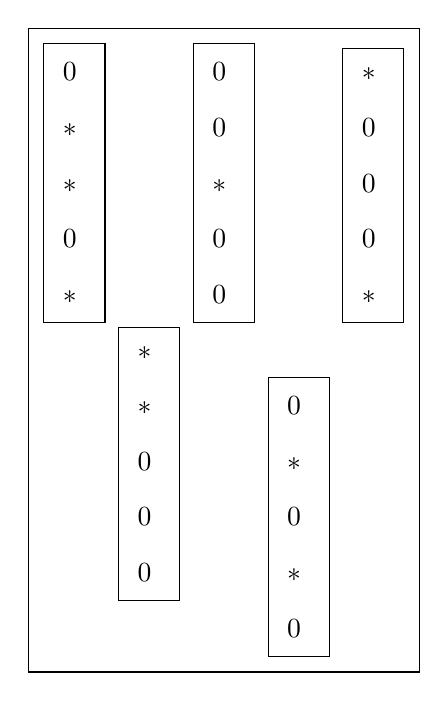
\begin{tikzpicture}[align=center, node distance=6cm]
						\matrix (cd) [
							matrix of nodes,
							draw=none,
							row sep = 0.7em,
							column sep = 1.2em,
							ampersand replacement=\&
						] {
							0                \& $\phantom{0}$    \& 0                \& $\phantom{0}$    \& $\s$          \\
							$\s$             \& $\phantom{0}$    \& 0                \& $\phantom{0}$    \& 0             \\
							$\s$             \& $\phantom{0}$    \& $\s$             \& $\phantom{0}$    \& 0             \\
							0                \& $\phantom{0}$    \& 0                \& $\phantom{0}$    \& 0             \\
							$\s$             \& $\phantom{0}$    \& 0                \& $\phantom{0}$    \& $\s$          \\
							$\phantom{0}$    \& $\s$             \& $\phantom{0}$    \& $\phantom{0}$    \& $\phantom{0}$ \\
							$\phantom{0}$    \& $\s$             \& $\phantom{0}$    \& 0                \& $\phantom{0}$ \\
							$\phantom{0}$    \& 0                \& $\phantom{0}$    \& $\s$             \& $\phantom{0}$ \\
							$\phantom{0}$    \& 0                \& $\phantom{0}$    \& 0                \& $\phantom{0}$ \\
							$\phantom{0}$    \& 0                \& $\phantom{0}$    \& $\s$             \& $\phantom{0}$ \\
							$\phantom{0}$    \& $\phantom{0}$    \& $\phantom{0}$    \& 0                \& $\phantom{0}$ \\
						};
						
						\visible<1> {
							\node[draw, fit = (cd-1-1) (cd-11-5), inner sep = 0.9em] (cd-fit) {};
						}
						
						\node[draw, fit = (cd-1-1) (cd-5-1)]  (c1) {};
						\node[draw, fit = (cd-1-3) (cd-5-3)]  (c3) {};
						\node[draw, fit = (cd-1-5) (cd-5-5)]  (c5) {};
						\node[draw, fit = (cd-6-2) (cd-10-2)] (c2) {};
						\node[draw, fit = (cd-7-4) (cd-11-4)] (c4) {};
					\end{tikzpicture}
				}
			}
			\only<3-> {
				\resizebox{0.9\textwidth}{!}{
					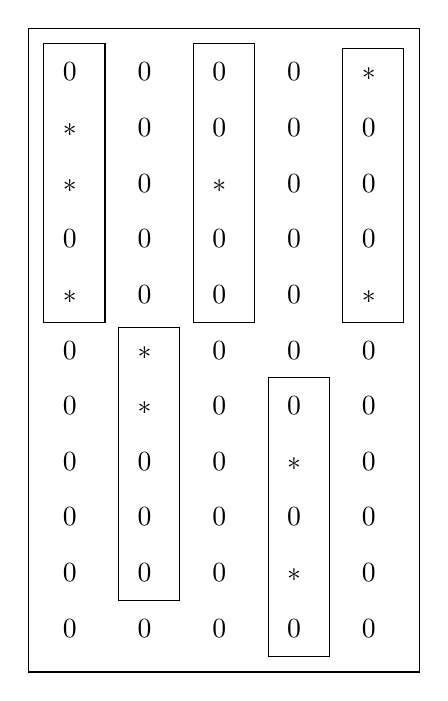
\begin{tikzpicture}[align=center, node distance=6cm]
						\matrix (cd) [
							matrix of nodes,
							draw=none,
							row sep = 0.7em,
							column sep = 1.2em,
							ampersand replacement=\&
						] {
							0    \& 0    \& 0    \& 0    \& $\s$ \\
							$\s$ \& 0    \& 0    \& 0    \& 0    \\
							$\s$ \& 0    \& $\s$ \& 0    \& 0    \\
							0    \& 0    \& 0    \& 0    \& 0    \\
							$\s$ \& 0    \& 0    \& 0    \& $\s$ \\
							0    \& $\s$ \& 0    \& 0    \& 0    \\
							0    \& $\s$ \& 0    \& 0    \& 0    \\
							0    \& 0    \& 0    \& $\s$ \& 0    \\
							0    \& 0    \& 0    \& 0    \& 0    \\
							0    \& 0    \& 0    \& $\s$ \& 0    \\
							0    \& 0    \& 0    \& 0    \& 0    \\
						};
						
						\node[draw, fit = (cd-1-1) (cd-11-5), inner sep = 0.9em] (cd-fit) {};
						
						\node[draw, fit = (cd-1-1) (cd-5-1)]  (c1) {};
						\node[draw, fit = (cd-1-3) (cd-5-3)]  (c3) {};
						\node[draw, fit = (cd-1-5) (cd-5-5)]  (c5) {};
						\node[draw, fit = (cd-6-2) (cd-10-2)] (c2) {};
						\node[draw, fit = (cd-7-4) (cd-11-4)] (c4) {};
					\end{tikzpicture}
				}
			}
		\end{column}
	\end{columns}
\end{frame}

\begin{frame}{Column Displacements --- Analysis}
	\begin{itemize}[<+->]
		\itemspacing{20pt}
		\item $m$ columns displacements to store
		\item $\O{n \log \log n + m}$ rows after displacements
		\item $\O{n}$ of them have nonnull row displacement
		\item Potential for more compression
	\end{itemize}
\end{frame}


\section{RDI Compression}
\begin{frame}{RDI Compression}
	\centering
	\resizebox{!}{0.75\textheight}{
		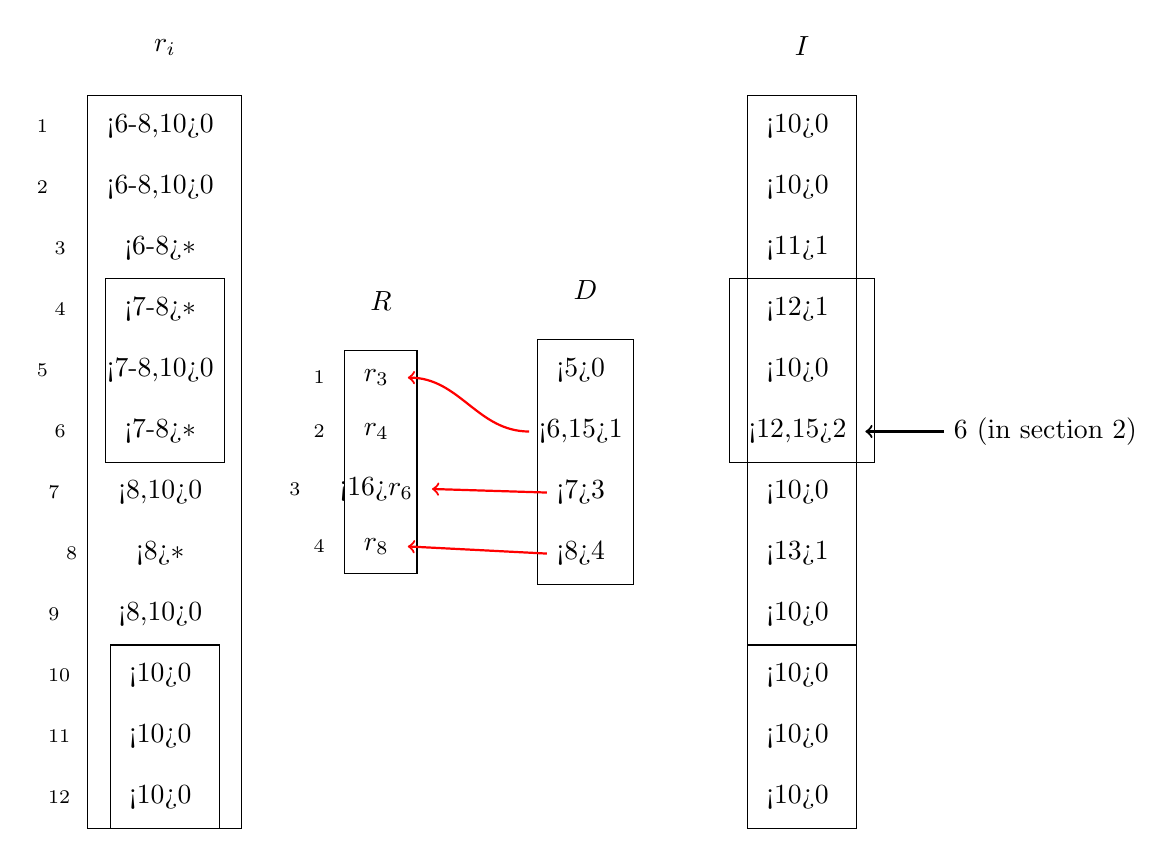
\begin{tikzpicture}[align=center, node distance=0.5cm and 1cm]
			\matrix (ri) [%
				matrix of nodes,
				draw = none,
				row sep = 0.7em,
				column sep = 0em
			]
			{
				\alert<6-8,10>{0}    \\
				\alert<6-8,10>{0}    \\
				\alert<6-8>{$\s$} \\
				\alert<7-8>{$\s$} \\
				\alert<7-8,10>{0}     \\
				\alert<7-8>{$\s$} \\
				\alert<8,10>{0}      \\
				\alert<8>{$\s$} \\
				\alert<8,10>{0}    \\
				\alert<10>{0}     \\
				\alert<10>{0}     \\
				\alert<10>{0}     \\
			};
			\node[draw, fit = (ri-1-1) (ri-12-1)] (ri-fit) {};
			\node[above = of ri-1-1] (rilabel) {$r_i$};
			
			\foreach \n in {1,...,12} {
				\node[font=\scriptsize, left = 0.5cm of ri-\n-1 ] {\n};
			}
			
			\visible<2->{
				\matrix (R) [%
					matrix of nodes,
					draw = none,
					row sep = 0.7em,
					column sep = 0em,
					right = of ri
				]
				{
					$r_3$ \\ $r_4$ \\ \alert<16>{$r_6$} \\ $r_8$ \\
				};
				\node[draw, fit = (R-1-1) (R-4-1)] (r-fit) {};
				\node[above = of R-1-1] (Rlabel) {$R$};
				
				\foreach \n in {1,...,4} {
					\node[font=\scriptsize, left = 0.25cm of R-\n-1 ] {\n};
				}
			}
			
			
			\visible<3->{
				\node[draw, fit = (ri-4-1) (ri-6-1)] (c) {};
				\node[draw, fit = (ri-10-1) (ri-12-1)] (d) {};
			}
			
			
			\visible<4->{
				\matrix (D) [%
					matrix of nodes,
					draw = none,
					row sep = 0.7em,
					column sep = 0em,
					right = of R
				]
				{
					\alert<5>{0} \\
					\alert<6,15>{1} \\
					\alert<7>{3} \\
					\alert<8>{4} \\
				};
				\node[draw, fit = (D-1-1) (D-4-1)] (D-fit) {};
				\node[above = of D-1-1] (Dlabel) {$D$};
			}
			
			\visible<6>{
				\draw[edge, red] (D-2-1.west) to[out=180, in=0] (R-1-1.east);
			}
				
			\visible<7>{
				\draw[edge, red] (D-3-1.west) to (R-3-1.east);
			}
				
			\visible<8>{
				\draw[edge, red] (D-4-1.west) to (R-4-1.east);
			}
			
			
			\visible<9->{
				\matrix (I) [%
					matrix of nodes,
					draw = none,
					row sep = 0.7em,
					column sep = 0em,
					right = of D
				]
				{
					\alert<10>{0} \\
					\alert<10>{0} \\
					\alert<11>{1} \\
					\alert<12>{1} \\
					\alert<10>{0} \\
					\alert<12,15>{2} \\
					\alert<10>{0} \\
					\alert<13>{1} \\
					\alert<10>{0} \\
					\alert<10>{0} \\
					\alert<10>{0} \\
					\alert<10>{0} \\
				};
				
				\node[draw, fit = (I-1-1) (I-12-1)] (i-fit) {};
				\node[above = of I-1-1] (Ilabel) {$I$};
				
				
				
				\node[draw, fit = (I-4-1) (I-6-1)] (a) {};
				\node[draw, fit = (I-10-1) (I-12-1)] (b) {};
			}
			
			
			\visible<14->{
				\node[right = 1cm of I-6-1] (lu6) {6 (in section 2)};
				\draw[edge] (lu6.west) to (I-6-1.east);
			}
			
		\end{tikzpicture}
	}
\end{frame}

\begin{frame}{RDI Compression}
	\begin{itemize}[<+->]
		\itemspacing{20pt}
		\item Values in $I$ are in $\O{\log \log n}$
		\item Pack multiple small values into one
		\item Reduces required storage for $I$
		\item Achieves overall compression of row displacements
	\end{itemize}
\end{frame}


\section{Combining Tries and Tables}
\begin{frame}{Putting Together the Pieces}
	\resizebox{\textwidth}{!}{%
		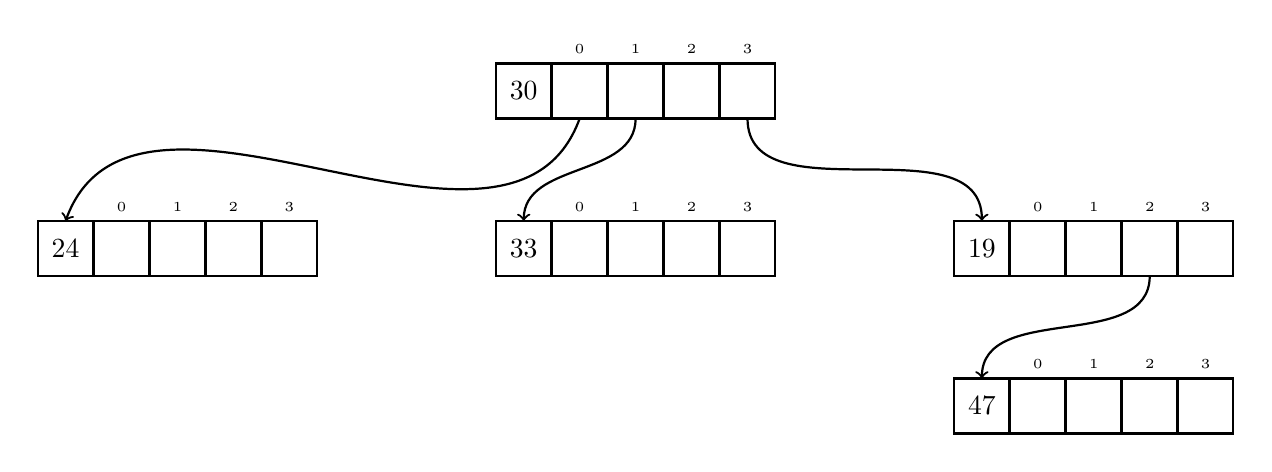
\begin{tikzpicture}[align=center, node distance=2cm]
			\trienode{30}{};
			
			\trienode{33}{below of=n30};
			\draw[edge] (n30-1-3.south) to[out=270, in=90] (n33-1-1.north);
		
			\trienode{24}{left =2cm of n33};
			\draw[edge] (n30-1-2.south) to[out=250, in=70] (n24-1-1.north);
		
			\trienode{19}{right=2cm of n33};
			\draw[edge] (n30-1-5.south) to[out=270, in=90] (n19-1-1.north);
		
			\trienode{47}{below of=n19};
			\draw[edge] (n19-1-4.south) to[out=270, in=90] (n47-1-1.north);
		\end{tikzpicture}
	}
\end{frame}
	
\begin{frame}{Putting Together the Pieces}
	\begin{itemize}[<+->]
		\itemspacing{20pt}
		\item Consider pointers as a table
		\item Compress this table as seen above
		\item In general: use trie with degree $n$
		\item Storage $\O{n}$ and access time $\O{\log_n N}$
		\item Special case: access time $\O{1}$ if $N \in \O{n^c}$
	\end{itemize}
\end{frame}


\begin{frame}
	\frametitle{\ }
	\begin{center}
		\LARGE Thank you for your attention!
	\end{center}
\end{frame}


\begin{frame}
	% empty frame
\end{frame}






\bibliographystyle{alpha}
\bibliography{literature}


\end{document}

